\documentclass{report}
\usepackage{geometry}
\usepackage{paralist}
\usepackage{scalerel,amssymb}
\usepackage{tikz}
\usepackage{pgfplots}
\usepackage{pgfplotstable}
\usepgfplotslibrary{fillbetween}
\usepackage{amsmath}
\usepackage{array}
\usepackage{nccmath}

\usepackage{fancyhdr}
\fancyhead[L]{\LARGE Applied Optimization \\
\Large Exercise 04}
\fancyhead[R]{13-123-922 \\
Elias \textsc{Wipfli} \\
13-933-262 \\
Lorenzo \textsc{Wipfli} \\
16-124-836 \\
Marcel \textsc{Zauder}}
\renewcommand{\headrulewidth}{0.4pt}
\fancyfoot[C]{\thepage}
\renewcommand{\footrulewidth}{0.4pt}

\definecolor{darkgreen}{rgb}{0.0, 0.4, 0.0}

\usepackage{hyperref}

\begin{document}
	\pagestyle{fancy}
	\hfill \\ \\
	
	\section*{4.1 Lagrange Duality}
	\subsection*{4.1.a}
	    The feasable set is the following:
	    \[
	       F \ = \ [x \mid x \in [2,4]] 
	    \]
	    The optimal value is: $x=2$, with $f_0(2) = 5$
	\subsection*{4.1.b}
	    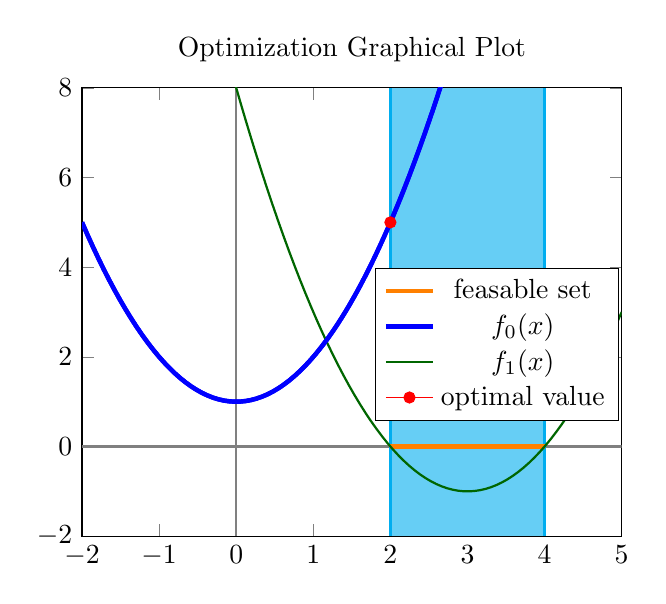
\begin{tikzpicture}
	        \begin{axis}[
		        title={Optimization Graphical Plot},
		        xmin = -2, xmax = 5, ymin = -2, ymax = 8,
		        domain=-2:5,
		        view={0}{90},
		        axis background/.style={fill=white},
		        legend style={at={(0.995,0.428)},anchor=east}
	        ]
	            \addplot[forget plot, color=gray, mark=none, thick] {0};
	            \addplot[forget plot, color=gray, mark=none, thick]  coordinates {(0,-2) (0,8) };
	            
	            %Line
		        \addplot[forget plot, color=cyan, thick] coordinates { (2,-2) (2,8) };
		        \addplot[forget plot, color=cyan, thick] coordinates { (4,-2) (4,8) };
		        \addplot[forget plot, color=black, name path=A] {8};
		        \addplot[forget plot, color=black, name path=B] {-2};
		        \addplot+[forget plot, cyan!60] fill between[of=A and B,soft clip={domain=2:4}];
		        \addplot[color=orange, mark=none, ultra thick, domain=2:4] {0};
	            
	            %Functions
		        \addplot[color=blue, mark=none, ultra thick, samples=100] {x^2 + 1};
		        \addplot[color=darkgreen, mark=none, thick, samples=100] {(x-2)*(x-4)};
		        \addplot[forget plot, color=blue, mark=none, ultra thick, samples=100] {x^2 + 1};
		        
		        %Nodes (Minima)
		        \addplot[mark=*, color=red] coordinates {(2,5)};
		        
		        %Legend
		        \addlegendentry{feasable set};
		        \addlegendentry{$f_0(x)$};
		        \addlegendentry{$f_1(x)$};
		        \addlegendentry{optimal value};
		        
	        \end{axis}
	    \end{tikzpicture}
	    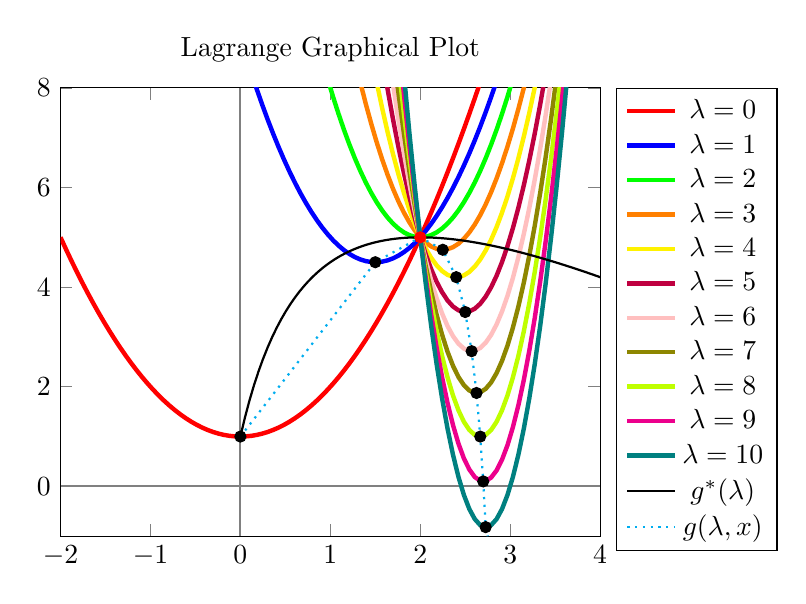
\begin{tikzpicture}
	        \begin{axis}[
		        title={Lagrange Graphical Plot},
		        xmin = -2, xmax = 4, ymin = -1, ymax = 8,
		        domain=-2:4,
		        view={0}{90},
		        axis background/.style={fill=white},
		        legend pos=outer north east,
	        ]
	            \addplot[forget plot, color=gray, mark=none, thick] {0};
	            \addplot[forget plot, color=gray, mark=none, thick]  coordinates {(0,-1) (0,8) };
	            
	            %Functions
		        \addplot[color=red, mark=none, ultra thick, samples=100] {x^2 + 1};
		        \addplot[color=blue, mark=none, ultra thick, samples=100] {2*x^2 - 6*x + 9};
		        \addplot[color=green, mark=none, ultra thick, samples=100] {3*x^2 - 12*x + 17};
		        \addplot[color=orange, mark=none, ultra thick, samples=100] {4*x^2 - 18*x + 25};
		        \addplot[color=yellow, mark=none, ultra thick, samples=100] {5*x^2 - 24*x + 33};
		        \addplot[color=purple, mark=none, ultra thick, samples=100] {6*x^2 - 30*x + 41};
		        \addplot[color=pink, mark=none, ultra thick, samples=100] {7*x^2 - 36*x + 49};
		        \addplot[color=olive, mark=none, ultra thick, samples=100] {8*x^2 - 42*x + 57};
		        \addplot[color=lime, mark=none, ultra thick, samples=100] {9*x^2 - 48*x + 65};
		        \addplot[color=magenta, mark=none, ultra thick, samples=100] {10*x^2 - 54*x + 73};
		        \addplot[color=teal, mark=none, ultra thick, samples=100] {11*x^2 - 60*x + 81};
		        \addplot[color=black, mark=none, thick, samples=100, domain=0:5]{((-1)*(x^2-9*x-1))/(x + 1)};
		        
		        %Line
		        \addplot[color=cyan, dotted, thick] coordinates { (0,1) (1.5,4.5) (2,5) (2.25,4.75) (2.4,4.2) (2.5,3.5) (2.571,2.714) (2.625,1.875) (2.667,1) (2.7,0.1) (2.727,-0.818) (2.75,-1)};
		        
		        %Nodes (Minima)
		        \addplot[mark=*] coordinates {(0,1)};
		        \addplot[mark=*] coordinates {(1.5,4.5)};
		        \addplot[mark=*, color=red] coordinates {(2,5)};
		        \addplot[mark=*] coordinates {(2.25,4.75)};
		        \addplot[mark=*] coordinates {(2.4,4.2)};
		        \addplot[mark=*] coordinates {(2.5,3.5)};
		        \addplot[mark=*] coordinates {(2.571,2.714)};
		        \addplot[mark=*] coordinates {(2.625,1.875)};
		        \addplot[mark=*] coordinates {(2.667,1)};
		        \addplot[mark=*] coordinates {(2.7,0.1)};
		        \addplot[mark=*] coordinates {(2.727,-0.818)};
		        
		        %Legend
		        \addlegendentry{$\lambda = 0$};
		        \addlegendentry{$\lambda = 1$};
		        \addlegendentry{$\lambda = 2$};
		        \addlegendentry{$\lambda = 3$};
		        \addlegendentry{$\lambda = 4$};
		        \addlegendentry{$\lambda = 5$};
		        \addlegendentry{$\lambda = 6$};
		        \addlegendentry{$\lambda = 7$};
		        \addlegendentry{$\lambda = 8$};
		        \addlegendentry{$\lambda = 9$};
		        \addlegendentry{$\lambda = 10$};
		        \addlegendentry{$g^*(\lambda)$};
		        \addlegendentry{$g(\lambda,x)$};
		        
	        \end{axis}
	    \end{tikzpicture}
	\subsection*{4.1.c}
	    Our start for the dual problem will look like the following function:
	    \[
	        g(\lambda) \ = \inf_{x \in D} [x^2 + 1 + \lambda (x-2)(x-4)]
	    \]
	    Now we compute the derivative of this function and the general solution for its minimum:
	    \begin{align*}
	        \bigtriangledown g( \lambda,x ) \ & = \ 2x + 2x\lambda - 6\lambda \\
	        \Rightarrow 2x + 2x\lambda - 6\lambda \ & = \ 0 \\
	        \Leftrightarrow x \ & = \ \frac{3\lambda}{1+\lambda}
	    \end{align*}
	    This value is now put into the function $g(\lambda, x)$ (calling it $g^*(\lambda)$, it is also plotted in the second plot):
	    \[
	        g^*(\lambda) \ = \ (\frac{3\lambda}{1+\lambda})^2 + 1 + \lambda (\frac{3\lambda}{1+\lambda} -2)(\frac{3\lambda}{1+\lambda} -4) \ = \ -\frac{(\lambda^2-9\lambda-1)}{\lambda+1}
	    \]
	    It is obvious that this function is concave and we need to find its maximum, so we compute the derivative and the extremum of this function:
	    \begin{align*}
	        \bigtriangledown g^*(\lambda) \ & = \ -\frac{\lambda ^2 + 2\lambda -8}{(\lambda +1)^2} \\
	        \Rightarrow -\frac{\lambda ^2 + 2\lambda -8}{(\lambda +1)^2} \ & = \ 0 \\
	        \Leftrightarrow \lambda ^2 + 2\lambda -8 \ & = \ 0 \\
	        \Leftrightarrow (\lambda + 4) \cdot (\lambda - 2) \ & = \ 0
	    \end{align*}
	    Because $\lambda > 0$, the result is 2. Because this is the exact optimal solution for x, the strong duality holds.
	\section*{4.2 KKT Condition}
	    The feasable set is like the following:
	    \[
	        F \ = \ [Point \ P(x_1,x_2) : x_1 + 4 = x_2, \ -10 \leq x_1 \leq -5 \ \vee -2 \leq x_1]
	    \]
	    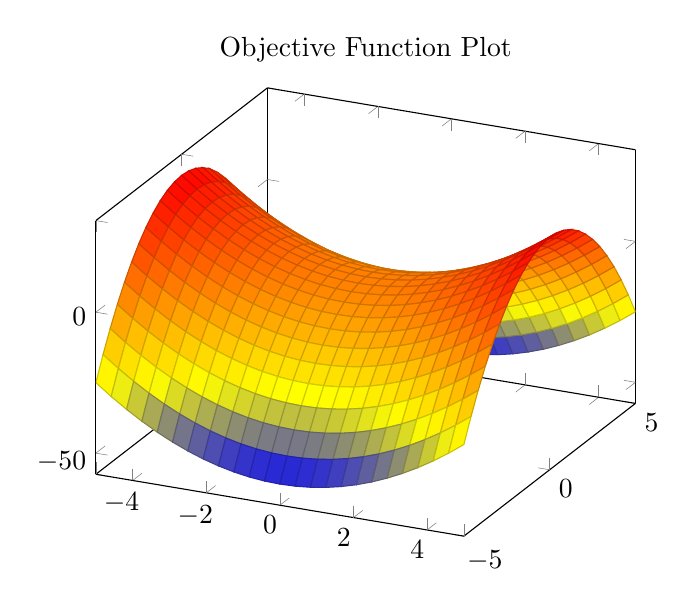
\begin{tikzpicture}
	        \begin{axis}[
	            title={Objective Function Plot},
	    ]
	            \addplot3[surf]{x^2 - 2*y^2};
	        \end{axis}
	    \end{tikzpicture}
	    \begin{tikzpicture}
	        \begin{axis}[
		        title={Graphical Plot},
		        xmin = -15, xmax = 50, ymin = -15, ymax = 50,
		        domain=-15:50,
		        view={0}{90},
		        axis background/.style={fill=white},
		        legend style={at={(0.995,0.12)},anchor=east}
	        ]
	            
	            \addplot[forget plot, color=gray, mark=none, thick] {0};
	            \addplot[forget plot, color=gray, mark=none, thick]  coordinates {(0,-15) (0,50) };
	            
	            %Functions
		        \addplot3[forget plot, contour gnuplot={number=40,labels=false}, samples=100, thick]{x^2 - 2*y^2};
		        \addplot[forget plot, domain=-12:5, color=blue, mark=none, ultra thick] {x^2 + 8*x + 14} node[below right, pos=0.7, text = black] {$f_1(x)$};
		        \addplot[forget plot, domain=-16:47, color=black, mark=none, ultra thick] {x + 4} node[below right, pos= 0.9, text = black] {$f_2(x)$};
		        \addplot[forget plot, color=red,mark=none, ultra thick]  coordinates {(-10,-15) (-10,50) } node[above right, pos=0, text = black] {$f_3(x)$};
		        \addplot[domain=-10:-5, color=darkgreen, mark=none, ultra thick]{x + 4};
		        \addplot[forget plot, domain=-2:47, color=darkgreen, mark=none, ultra thick]{x + 4};
		        
		        %Nodes
		        \addplot[mark=*, color=darkgreen] coordinates {(-10,-6)};
		        \addplot[mark=*, color=darkgreen] coordinates {(-5,-1)};
		        \addplot[mark=*, color=darkgreen] coordinates {(-2,2)};
		        
		        %Legend
		        \addlegendentry{feasable set};
		        \addlegendentry{critical points};
		        
	        \end{axis}
	    \end{tikzpicture}
	    \hfill \\ \\
	    Because we can see that the optimal solution must be on the function $f_2(x) = x_1 + 4$ and the further we go on it the smaller the value of the objective function becomes (because the contour lines are getting "bluish"), its values for $x_1$ and $x_2$ will get to $\infty$ and therefore its solution will be $-\infty$. This solution does not satisfy the KKT conditions.
	\section*{4.3 Programming}
	
\end{document}